\documentclass{ltjsarticle}
%%%package読み込み
\usepackage{amsmath}
\usepackage{amssymb}
\usepackage{amsfonts}
\usepackage{mathtools}
\usepackage{bm}
% \usepackage{tikz} % ★消去: 代わりに graphicx 追加
% \usetikzlibrary{cd}
\usepackage{url}
\usepackage{graphicx} % ★追加: 図を挿入するため
\usepackage{float} % ★追加: 図の位置を制御するため
\usepackage{caption} % ★追加: 図のキャプションを柔軟に扱うため
%\usepackage{xcolor}
\usepackage{ascmac}
\usepackage{tcolorbox}
%\usepackage[dvipdfmx, setpagesize=false, bookmarks=true, bookmarksdepth=tocdepth, bookmarksnumbered=true, colorlinks=true, linkcolor=red]
\usepackage{hyperref}
\usepackage[version=4]{mhchem}
\usepackage{braket} % 追加した
\usepackage{booktabs}
\usepackage{bookmark}
%\usepackage{pxjahyper}
%%%黒板太字
\newcommand{\N}{\mathbb{N}}
\newcommand{\Z}{\mathbb{Z}}
\newcommand{\Q}{\mathbb{Q}}
\newcommand{\R}{\mathbb{R}}
\newcommand{\C}{\mathbb{C}}
\newcommand{\F}{\mathbb{F}}
%%%約物
\newcommand{\abs}[1]{\left|#1\right|}
\newcommand{\lr}[1]{\left(#1\right)}
\newcommand{\st}{\; \mathrm{s.t.}\; }
\newcommand{\Ae}{\textrm{-a.e.}} 
%%%繰り返し
\newcommand{\pluss}[3]{#1_{#2}+\cdots+#1_{#3}}
\newcommand{\minuss}[3]{#1_{#2}-\cdots-#1_{#3}}
\newcommand{\timess}[3]{#1_{#2}\times\cdots\times #1_{#3}}
\newcommand{\leqs}[3]{#1_{#2}\leq\cdots\leq #1_{#3}}
\newcommand{\geqs}[3]{#1_{#2}\geq\cdots\geq #1_{#3}}
\newcommand{\opluss}[3]{#1_{#2}\oplus\cdots\oplus #1_{#3}}
\newcommand{\otimess}[3]{#1_{#2}\otimes\cdots\otimes #1_{#3}}
\newcommand{\commas}[3]{#1_{#2},\ldots,#1_{#3}}
%%%微分
\newcommand{\dx}[1]{\mathrm{d}#1}
\newcommand{\ddx}[1]{\frac{\mathrm{d}}{\mathrm{d}#1}}
\newcommand{\dydx}[2]{\frac{\mathrm{d}#1}{\mathrm{d}#2}}
\newcommand{\dydxn}[3]{\frac{\mathrm{d}^{#3}#1}{\mathrm{d}#2^{#3}}}
\newcommand{\del}[2]{\frac{\partial#1}{\partial#2}}
\newcommand{\dell}[2]{\frac{\partial^2#1}{{\partial#2}^2}}
\newcommand{\deln}[3]{\frac{\partial^{#3}#1}{{\partial#2}^{#3}}}
%%%
%%%演算子
%log type
\let\Re\relax
\DeclareMathOperator{\Re}{Re}
\let\Im\relax
\DeclareMathOperator{\Im}{Im}
\DeclareMathOperator{\sgn}{sgn}
\DeclareMathOperator{\sign}{sign}
\DeclareMathOperator{\Supp}{Supp}
\DeclareMathOperator{\tr}{tr}
\DeclareMathOperator{\Tr}{Tr}
\DeclareMathOperator{\Det}{Det}
\DeclareMathOperator{\Log}{Log}
\DeclareMathOperator{\rank}{rank}
\DeclareMathOperator{\diag}{diag}
\DeclareMathOperator{\corank}{corank}
\DeclareMathOperator{\Res}{Res}
\DeclareMathOperator{\Ker}{Ker}
\DeclareMathOperator{\coker}{coker}
\DeclareMathOperator{\Coker}{Coker}
\DeclareMathOperator{\Var}{Var}
\DeclareMathOperator{\Cov}{Cov}
\DeclareMathOperator{\sech}{sech}
\DeclareMathOperator{\csch}{csch}
\DeclareMathOperator{\arcsec}{arcsec}
\DeclareMathOperator{\arccot}{arccot}
\DeclareMathOperator{\arccsc}{arccsc}
\DeclareMathOperator{\arccosh}{arccosh}
\DeclareMathOperator{\arcsinh}{arcsinh}
\DeclareMathOperator{\arctanh}{arctanh}
\DeclareMathOperator{\arcsech}{arcsech}
\DeclareMathOperator{\arccsch}{arccsch}
\DeclareMathOperator{\arccoth}{arccoth}
\DeclareMathOperator{\grad}{grad}
\let\div\relax
\DeclareMathOperator{\div}{div}
\DeclareMathOperator{\rot}{rot}
%\DeclareMathOperator{\GL}{GL} % ★消去 : ここから↓
%\DeclareMathOperator{\SL}{SL}
%\DeclareMathOperator{\Sym}{Sym}
%\DeclareMathOperator{\Aut}{Aut}
%\DeclareMathOperator{\Inn}{Inn}
%\DeclareMathOperator{\Out}{Out}
%\DeclareMathOperator{\id}{id}
%\DeclareMathOperator{\pr}{pr}
%\DeclareMathOperator{\supp}{supp}
%\DeclareMathOperator{\diam}{diam}
%\DeclareMathOperator{\End}{End}
%\DeclareMathOperator{\Cl}{Cl}
%\DeclareMathOperator{\Hom}{Hom} % ★消去 : ここまで↑
%limit type
\DeclareMathOperator*{\argmin}{arg~min}
\DeclareMathOperator*{\argmax}{arg~max}
%%%
%%%定理
\usepackage{amsthm}
\theoremstyle{definition}
\newtheorem{lem}{補題}
\newtheorem*{lem*}{補題}
\newtheorem{prf}{証明}
\newtheorem*{prf*}{証明}
\newtheorem*{ex*}{Example}
\newtheorem*{rem*}{Remark}
\newenvironment{prb}[1]%
{\begin{itembox}[l]{\textbf{問題 #1}}}%
{\end{itembox}}
\newenvironment{sol}[2]%
{\setcounter{lem}{0}
\setcounter{prf}{0}
\par\noindent\textbf{解答 #1} (#2)\par}%
{\par\normalfont}

\renewcommand{\refname}{Reference}


%%%%%%%%%%%%%%%%%%%%%
\numberwithin{equation}{section}
%%%%%%%%%%%%%%%%%%%%%%

\newcounter{boxeddefcounter}
\newenvironment{problem}
{\refstepcounter{boxeddefcounter}\begin{itembox}[l]{問\theboxeddefcounter}}
{\end{itembox}}

%\usepackage[hang,small,bf]{caption}
%\usepackage[subrefformat=parens]{subcaption}
\captionsetup{compatibility=false}


\newcommand{\D}{^\circ\text{C}}
\newcommand{\ka}{\textasciitilde}


\pagestyle{myheadings}
\begin{document}
%%タイトル
\title{Organic experiment Unit.5}
\date{実験日: 7/16, 17, 22, 10/2, 6}
\author{実験者: No.7 05253011 Fumiya Kashiwai / 柏井史哉}
\maketitle
\markboth{Organic experiment Unit.5 No.7 05253011 Fumiya Kashiwai / 柏井史哉} {Organic experiment Unit.5 No.7 05253011 Fumiya Kashiwai / 柏井史哉}
%%ここまでタイトル

\section{未知試料の分離、同定}
\subsection{Purpose and Background}
2種類の有機化合物の混合物を、化学的性質を用いて分離、精製する。また、精製した試料に対して官能基試験を行うとともに物性や分光学的スペクトルを取得し、化合物を同定する。

\subsection{Experimental}
\subsubsection{未知資料の分離}
\begin{enumerate}
\item 外観を観察すると、薄黄色の板状結晶の固体 (\textbf{A}) と、白色の針状結晶の混合物 (\textbf{B}) であった。スパチュラを用いて大まかに分離した。
\item 荒く分離したそれぞれの試料のhexane、DCM、\ce{Et2O}への溶解度を調べた。
\item それぞれのDCM溶液をTLC展開 (hexane: \ce{EtOAc} = 2:1) した。\textit{p-}anisaldehydeを噴射し、加熱して呈色の様子を調べた。
\item \textbf{A}、\textbf{B}の混合物を試験管に微量取り、1M \ce{NaOH}\textit{aq.}と DCMをそれぞれ1 mL程度加えて振盪した。各層の溶液をTLC展開 (hexane: \ce{EtOAc} = 2:1) した。
\item 荒く分離した\textbf{B} を\ce{Et2O} 10 mLに溶解し、10 mLの1M \ce{NaOH}\textit{aq.} で2回抽出した。水層を集めて1M \ce{HCl}\textit{aq.}で中和したところ白色固体が析出した。
\item 水層から析出した白色固体を吸引濾過、水で洗浄、風乾した。
\item エーテル層を少量のBrineで洗浄し、無水\ce{MgSO4}により乾燥し、溶媒をエバポレーターで減圧 ($35\D$/300 mmHg) して除去した。
\item 精製した\textbf{A}、\textbf{B}の融点を測定したところ、\textbf{A}は$54-55\D$ 、\textbf{B}は$163-164\D$
であった。
\item IRスペクトル (nujol)、\ce{^1H} NMRスペクトルを測定した。それぞれfig.\ref{NMR_5-1-A} - \ref{IR_5-1-B} に示す。
\end{enumerate}

\subsubsection{官能基試験}
\begin{enumerate}
\item 精製した\textbf{A}、\textbf{B} 10 mg程度をそれぞれ極少量の\ce{MeOH}に溶解し、Brady試薬を加え、振盪したところ、\textbf{A}は変化がなく、\textbf{B}では赤色沈澱が生じた。
\item \textbf{A} 0.05 gをアセトン0.5 mLに溶解し、1\% \ce{KMnO4} を1滴滴下し、数分放置したが脱色は生じなかった。
\item 濃\ce{H2SO4} 10滴に、スパチュラ1杯の\textbf{A}を加えると溶解し、黄色い溶液となった。
\end{enumerate}

\subsubsection{\textbf{A}の誘導体の合成}
\begin{enumerate}
\item スターラーを入れた30 mLフラスコに濃\ce{HCl}\textit{aq.} 1mLを加えた。
\item \ce{SnCl2} 0.54 g、\textbf{A} 0.05 gを加えた。
\item 撹拌しながら$70\D$のオイルバスで10 min還流した。
\item TLCで還元反応の完了を確認し、加熱を終了、粒状の\ce{NaOH}を加えたところ白濁した。pH試験紙を用いてpHを測定するとpH = 11であった。
\item \ce{Et2O} 10 mLにより3回抽出を行った。
\item \ce{Et2O}層を合わせるとやや白濁していた。水20 mLを用いて洗浄すると水層が白濁し、\ce{Et2O}層の白濁が薄まった。
\item Brine 20 mLを用いて\ce{Et2O}層を洗浄し、無水\ce{MgSO4}を加えて乾燥し、濾過して除去した。
\item エバポレーターで溶媒を除去し、黄色い結晶を得た。得た固体の融点は$45 - 47\D$であった。また、R$_f$ = 0.68 (hexane : AcOEt = 2:1) であった。
\item \ce{^1H} NMRスペクトルを測定した。測定結果はfig. \ref{NMR_5-1-A-2}に示す。
\end{enumerate}
\subsection{Results and Discussion}
溶媒への溶解度は、table.\ref{solubility}に示したようになった。
また、TLC展開において、UV照射下で$R_f = 0.87$にピンク色、$R_f = 0.17$に青色のスポットが呈色した。どちらのピークも\textit{p-}anisaldehydeの噴射、加熱によっては呈色しなかった。
荒く分離した試料において、試料\textbf{A}では$R_f = 0.87$のみが、試料\textbf{B}では$R_f = 0.87, 0.17$の双方が確認された。試料\textbf{A}はほぼ純粋に分離できているが、荒く分離した試料\textbf{B}には\textbf{A}がコンタミネーションしていたと考えられる。
\begin{table}[htp]
\caption{\textbf{A}, \textbf{B}の溶媒への溶解度}
\begin{center}
\begin{tabular}{ccc}
\toprule
solvent & \textbf{A} & \textbf{B} \\
\midrule
hexane & 難溶 & 難溶\\
DCM & 可溶 & 難溶\\
\ce{Et2O} & 可溶 & 可溶\\
\bottomrule
\end{tabular}
\end{center}
\label{solubility}
\end{table}%

\ce{NaOH}\textit{aq.}と\ce{Et2O}による分離操作では、UV照射下で油層に$R_f = 0.87$、水層では原点にとどまるスポットが呈色した。これより、油層には\textbf{A}が留まり、水層には\textbf{B}が塩として移動したと考えられる。また、これより\ce{NaOH}\textit{aq.}と\ce{Et2O}により分離が可能であることが確認できた。

\ce{^1H} NMRスペクトルでは、試料\textbf{A}の芳香族領域に2本のdoublet (積分比がそれぞれ2程度) が見られることから、芳香族の\textit{p-}2置換体と考えられる。
また、2.46 ppmのsinglet (積分比3.26) はメチル基の存在を示唆し、tolueneの\textit{p-}置換体と考えられる。
1.53 ppmのピークは溶媒の水に帰属される\cite{nmr_solvent}。試料\textbf{A}にこれ以外の水素は存在しないと考えられる。
IRスペクトルで1524 cm$^{-1}$に中程度の吸収が見られ、試料\textbf{A}は\textit{p-}nitro-toluene (fig.\ref{structure} の化合物\textbf{1}) と推測した。

\ce{SnCl2}を用いて試料\textbf{A}を還元すると\textit{p-}amino-toluene (\textit{p-}toluidine) が生成すると期待される。実際、合成した化合物の融点は$45-47\D$ (文献値: $45\D$) であり、\ce{^1H} NMRスペクトル (fig. \ref{NMR_5-1-A-2}) も\textit{p-}toluidineの構造を支持する。

具体的には、6.61 ppm, 6.96 ppmにそれぞれ存在するdoublet は芳香族領域の中では高磁場であり、電子供与基の存在が示唆される。また、3.52 ppmのbroadした2Hは、アミノ基に帰属される。

さらに、反応終了後の酸性条件から塩基性条件に変えると白濁したことから、塩基性のアミノ基の存在が示唆される。

以上から\textbf{A}を\textit{p-}nitro-tolueneと同定した。

\textbf{B}では、Brady試薬で赤色の沈澱が見られたことから、カルボニル基の存在が示唆される。\ce{^1H} NMRスペクトル (fig. \ref{NMR_5-1-B}) の芳香族領域の4Hのカップリングより、\textit{o-}2置換体であると考えられる。また、6.94 ppm, 7.01 ppmの2Hは比較的高磁場であり、電子供与基の存在が示唆される。反面、7.9 ppm程度の2Hは比較的低磁場であり、電子吸引基の存在が示唆される。Brady試験と合わせ、安息香酸の\textit{o-}置換体であると予測される。

融点の測定値$163-164\D$はサリチル酸の文献値: $162-165\D$ とよく一致する。
2.5 ppm付近に非常になだらかなシグナルが見られる。サリチル酸では分子内および分子間水素結合を形成すると考えられ、ヒドロキシ基およびカルボニル酸の\ce{H}が10.45 ppm、2.5 ppm程度に出現している可能性がある。今回は\ce{CDCl3}を溶媒として用いたが、\ce{DMSO}を用いることで水素結合の影響を抑えてシャープなスペクトルを得られる可能性がある\cite{Abrahum}。

そのほかのピークを含め、帰属結果をfig.\ref{NMR_5_attiribute}に示した。IRスペクトルについても、table.\ref{IR_5-A_attribute} および table.\ref{IR_5-B_attribute} に示した。
\begin{figure}[htbp]
\begin{center}
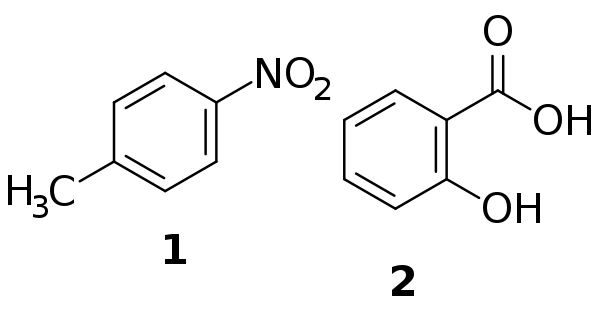
\includegraphics[width = 8 cm]{structure5-1.png}
\caption{同定した構造}
\label{structure}
\end{center}
\end{figure}

\section{誘導体の合成}
\subsection{Purpose and Background}
精製したサリチル酸から誘導体を合成し、安定な結晶性物質を得る。誘導体の物性、スペクトルにより同定を行う。
\begin{figure}[htbp]
\begin{center}
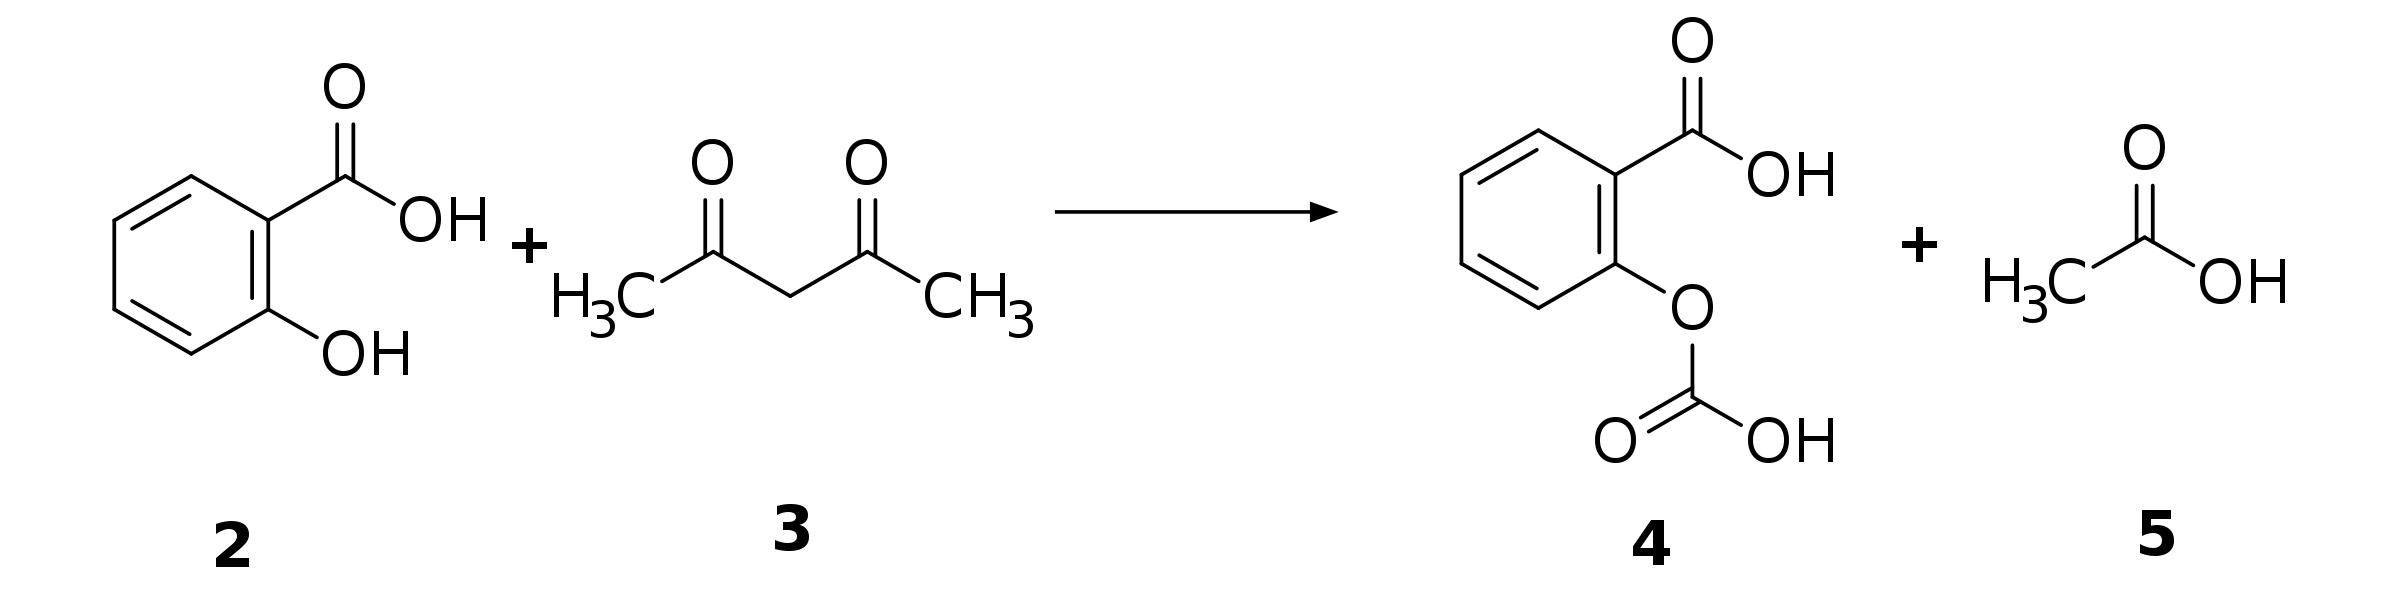
\includegraphics[width = 15 cm]{reaction5-1.png}
\caption{誘導体の合成スキーム}
\label{scheme5-1}
\end{center}
\end{figure}

アセチル化により結晶性のアセチルサリチル酸を得ることができる\cite{Zhong}。


\subsection{Experimental}
\paragraph{First Try}
\begin{enumerate}
\item day3までに精製した化合物\textbf{2} 0.37 gを50 mLフラスコにとり、化合物\textbf{3} 3 mLを滴下した。
\item 濃硫酸を2滴滴下したところ、発熱を伴いながら無色透明から黄色がかった透明溶液に変化した。
\item TLCで反応の進行を15分後に確認し、水20 mL程度を加えたのち\ce{NaHCO3}粉末を、発泡が止まるまで加え、pHが8程度であることを確認した
\item 分液ロートに移し、さらに水を30 mL程度加えて固体を完全に溶解させた。\ce{EtOAc}を 50 mL程度加え、分液操作を行なった。
\item 得られた\ce{EtOAc}層をBrine 20 mLで洗浄した。
\item 無水\ce{Na2SO4}を加え乾燥し、濾過により除いた。
\item 得られた\ce{EtOAc}層をエバポレーター (70 mmHg / 35$\D$)にかけ、溶媒を除去した。
\item なすフラスコの壁面に微量の白色結晶を認めた。これをごく少量のEtOAcに溶解し、TLCを行なった。
\end{enumerate}
\paragraph{Second Try}
\begin{enumerate}
\item 純粋な化合物\textbf{2} 0.10 gを50 mLフラスコにとり、化合物\textbf{3} 3 mLを滴下した。
\item 濃硫酸を2滴滴下したところ、発熱を伴いながら無色透明から黄色がかった透明溶液に変化した。
\item 15分後に水20 mL程度を加えたのち\ce{NaHCO3}粉末を、発泡が止まるまで加え、pH~8であることを確認した
\item 分液ロートに移し、さらに水を30 mL程度加えて固体を完全に溶解させた。\ce{EtOAc}を 50 mL程度加え、分液操作を行なった。
\item 得られた\ce{EtOAc}層をBrine 20 mLで洗浄した。
\item 無水\ce{Na2SO4}を加え乾燥し、濾過により除いた。
\item 得られた\ce{EtOAc}層をエバポレーター (100 mmHg / 35$\D$)にかけ、溶媒を除去した。
\item 得られた微量の白色固体の融点の測定値は、$132-134\D$ (文献値: $135\D$) であった。
\end{enumerate}
\subsection{Results and Discussion}
TLC (展開溶媒 hexane : AcOEt = 2 : 1)でアセチル化を追跡した。15 minの反応後、出発物のスポット ($R_f = 0.55$)は消失し、新たな単一のスポット ($R_f = 0.45$) が出現した。両者はUV照射下で呈色した。硫酸の滴下により発熱が生じるとともに色の変化が見られることから、反応は極めて迅速に進行し、スターラーによる撹拌なしでも15 minで完全に反応が進行すると考えられる。
得られた結晶の融点は132 - 134$\D$ (化合物\textbf{3}の文献値: 135$\D$)であり、文献値と概ね一致していた。これよりアセチルサリチル酸\textbf{4}が高純度で合成できたと考えられる。しかしながら精製物は微量であり、収率は好ましくなかった。また、First Tryでは化合物\textbf{4}が得られなかった。

収率が低かった要因としてはまず分液操作が不完全であった可能性があげられる。有機層への抽出が1回のみでは不十分であった可能性が高い。水層と有機層をTLCで適宜モニターしながら抽出回数を決定すべきであった。

それに加え、一回めの試行では7月に精製し、実験室に放置したサンプルを用いたため劣化していた可能性がある。
%\subsection{Discussion}
%%参考文献
\begin{thebibliography}{99}
\bibitem{nmr_solvent}
Hugo E. Gottlieb, Vadim Kotlyar, and
Abraham Nudelman, 
NMR Chemical Shifts of Common
Laboratory Solvents as Trace Impurities
\textit{J. Org. Chem.}  \textbf{1997}, 62, 7512-7515.
\bibitem{Zhong}
Zhong-Duo Yang, Zhu-Wen Song, Jin Ren, Ming-Jun Yang, Shuo Li.
Improved Thin-layer Chromatography Bioautographic Assay for the Detection of Acetylcholinesterase Inhibitors in Plants.
Phytochemical Analysis. \textbf{2011}, 22(6), 509-515.
\bibitem{Abrahum}
Michael H. Abraham, Raymond J. Abraham, William E. Acree, Jr., Abil E. Aliev, Al J. Leo, William L. Whaley. 
An NMR Method for the Quantitative Assessment of Intramolecular Hydrogen Bonding; Application to Physicochemical, Environmental, and Biochemical Properties.
\textit{J. Org. Chem.} \textbf{2014}, 79, 22, 11075-11083
\end{thebibliography}

\clearpage

%\subsection{Conclusion}
\section{Appendix}
\begin{figure}[htbp]
\begin{center}
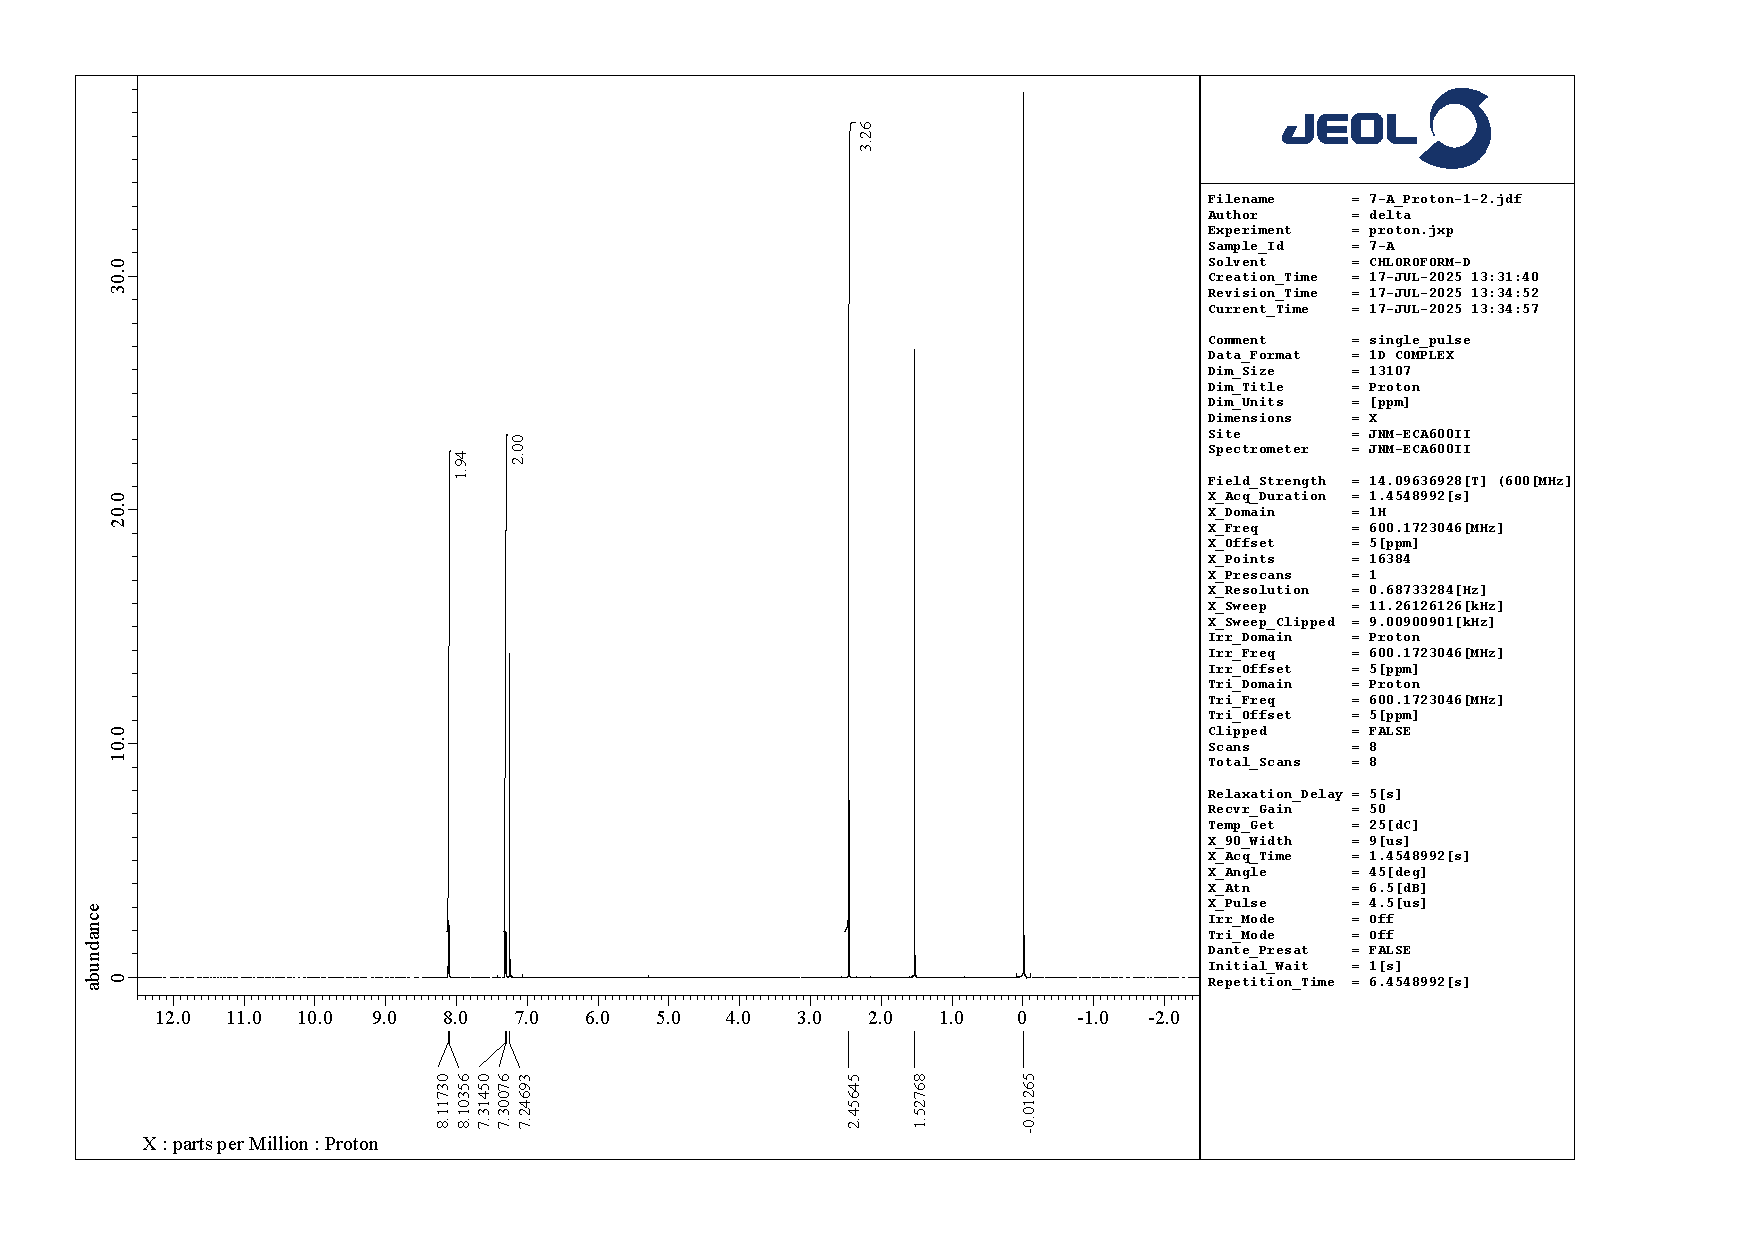
\includegraphics[width = 15 cm]{NMR_5-1-A.pdf}
\caption{\textbf{A}の\ce{^1H} NMRスペクトル (\ce{CDCl3})}
\label{NMR_5-1-A}
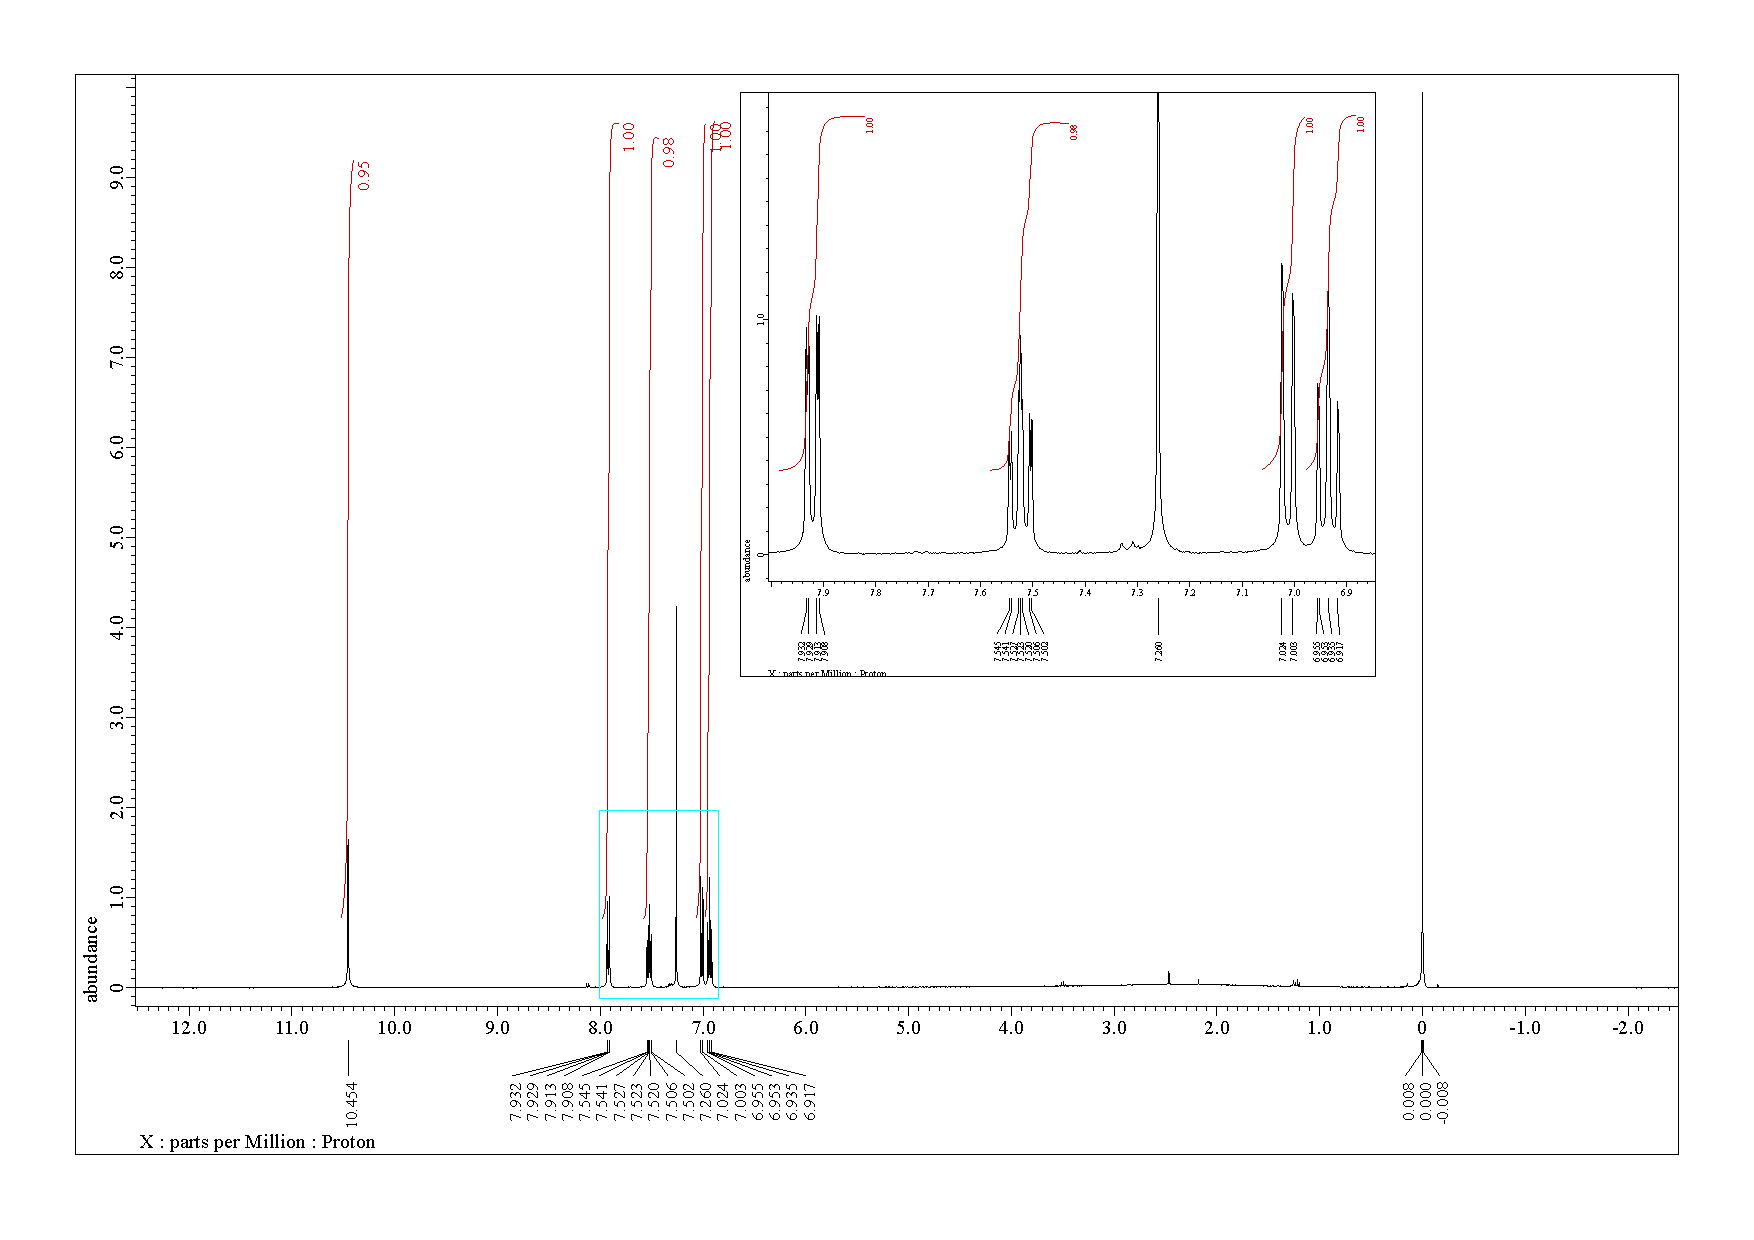
\includegraphics[width = 15 cm]{NMR_5-1-B.pdf}
\caption{\textbf{B}の\ce{^1H} NMRスペクトル (\ce{CDCl3})}
\label{NMR_5-1-B}
\end{center}
\end{figure}
\begin{figure}[htbp]
\begin{center}
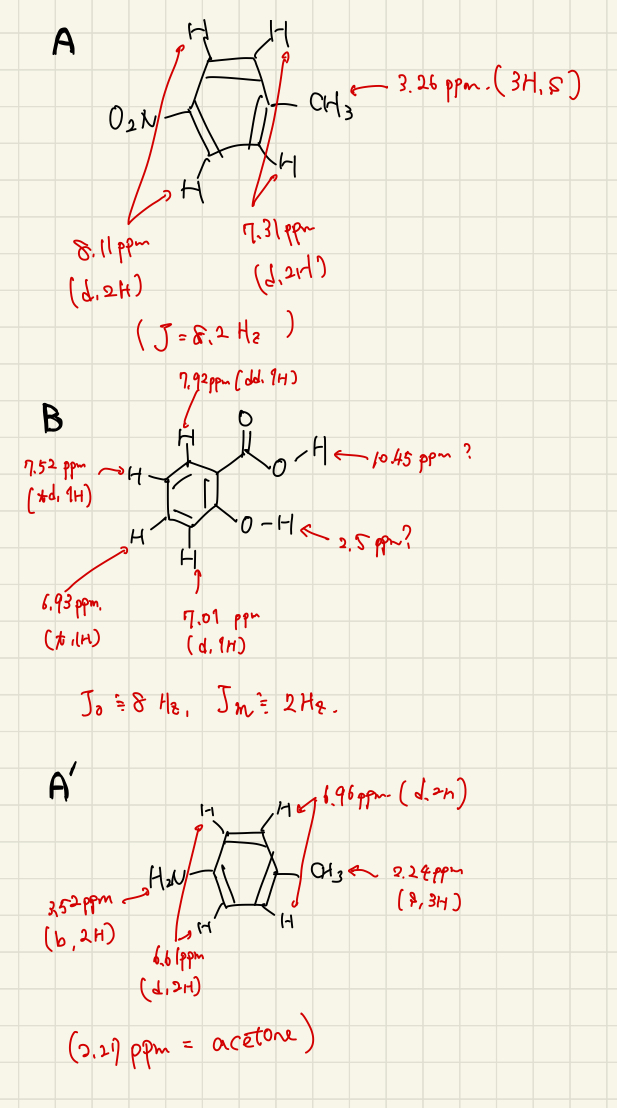
\includegraphics[width = 10 cm]{NMR_5_attribute.jpeg}
\caption{NMRスペクトルの帰属}
\label{NMR_5_attiribute}
\end{center}
\end{figure}



\begin{figure}[htbp]
\begin{center}
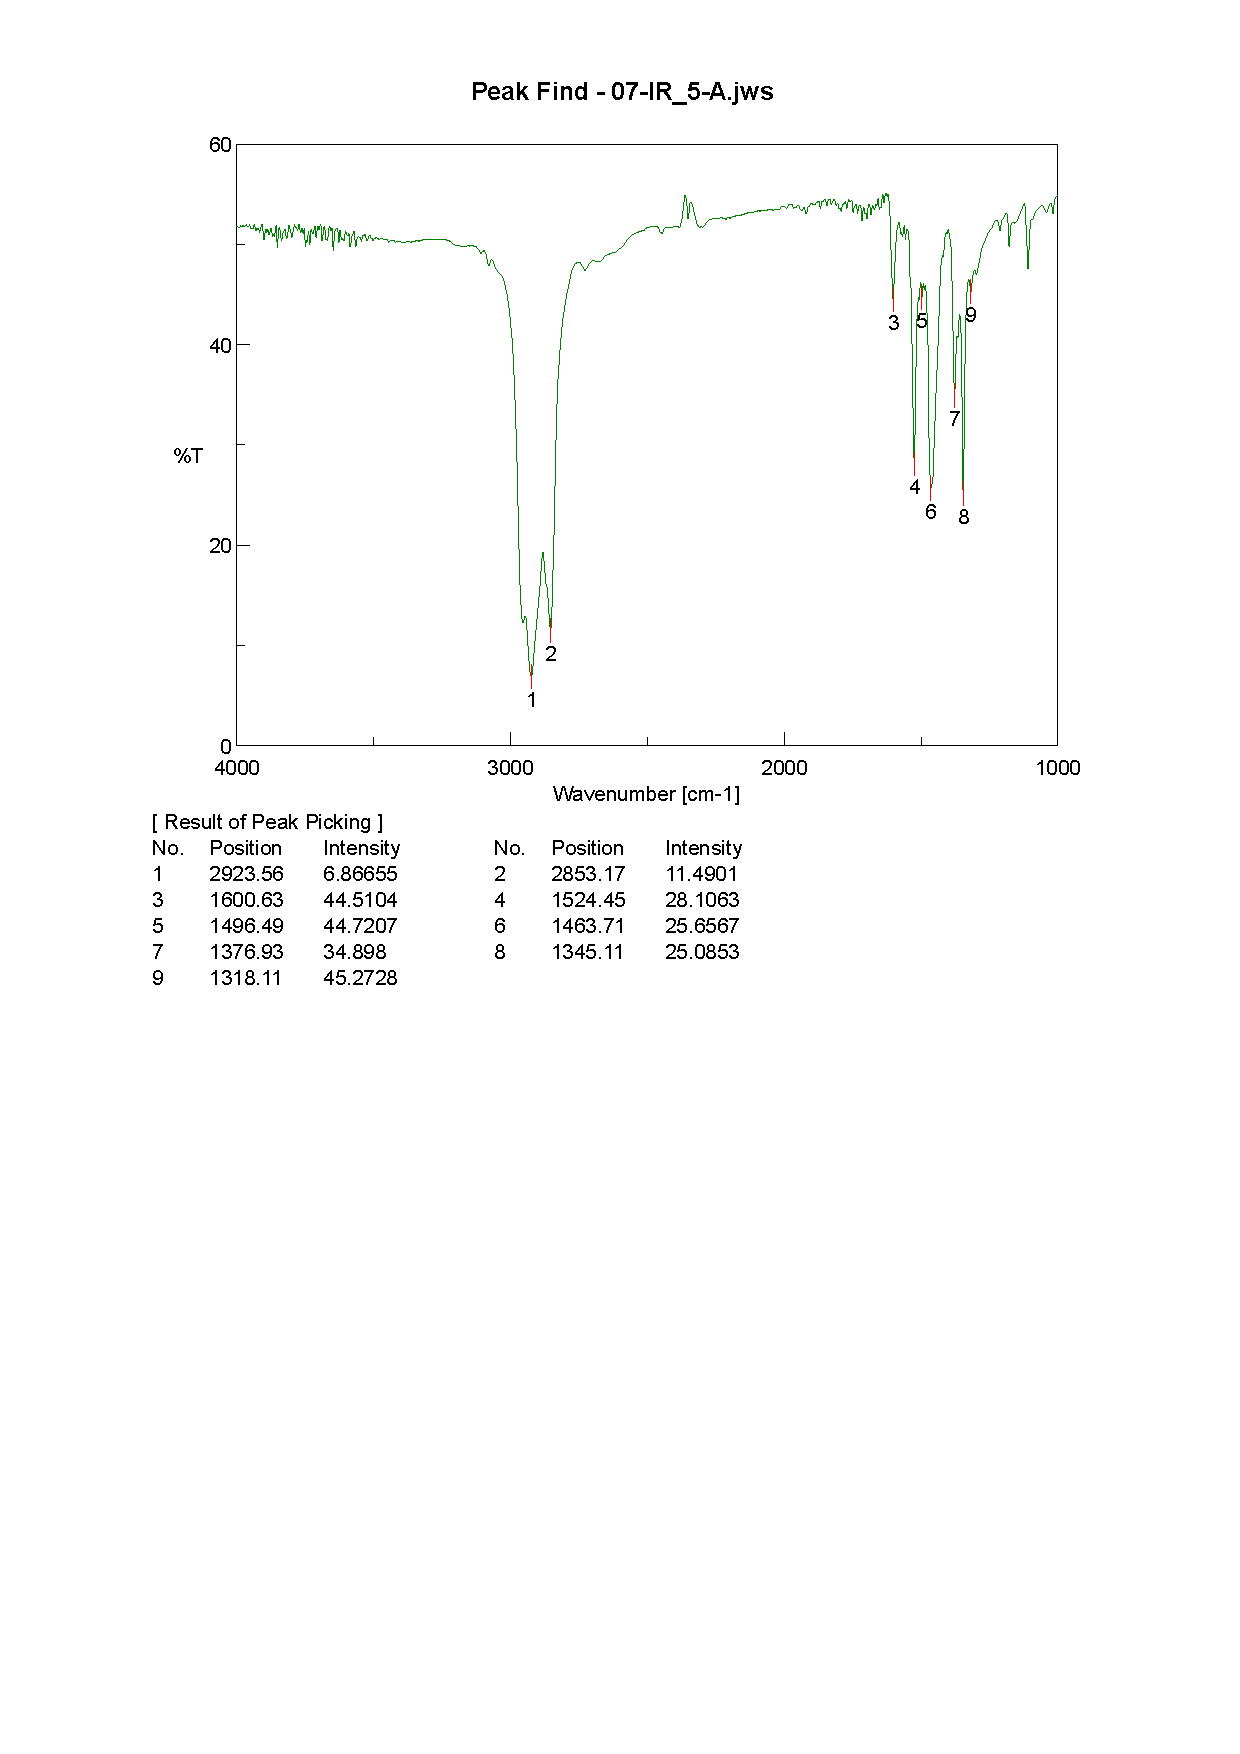
\includegraphics[width = 15 cm]{IR_5-1-A.pdf}
\caption{IR:5-1-A}
\label{IR_5-1-A}
\end{center}
\end{figure}

\begin{table}[htp]
\caption{IR: 5-A の帰属}
\begin{center}
\begin{tabular}{cc cc}
\toprule
No. & Wavenumber [cm-1] & Intensity & attribution \\
\midrule
1 & 2923 & strong & nujol\\
2 & 2853 & strong & nujol\\
3 & 1601 & mid & \\
4 & 1524 & strong & \ce{N-O} stretch\\
5 & 1496 & weak & \\
6 & 1464 & strong  & nujol\\
7 & 1376 & mid &  \ce{N-O} stretch\\
8 & 1345 & strong & nujol?\\
9 & 1318 & weak & nujol?\\
\bottomrule
\end{tabular}
\end{center}
\label{IR_5-A_attribute}
\end{table}%

\begin{table}[htp]
\caption{IR: 5-B の帰属}
\begin{center}
\begin{tabular}{cc cc}
\toprule
No. & Wavenumber [cm-1] & Intensity & attribution \\
\midrule
1 & 2953 & strong & C-H stretch (芳香族)?\\
2 & 2924 & strong & nujol\\
3 & 2853 & strong & nujol\\
4 & 1660 & mid & \ce{C=O} stretch\\
5 & 1612 & mid & ?\\
6 & 1463 & strong & nujol\\
7 & 1377 & mid  & nujol\\
\bottomrule
\end{tabular}
\end{center}
\label{IR_5-B_attribute}
\end{table}%

\begin{figure}
\begin{center}
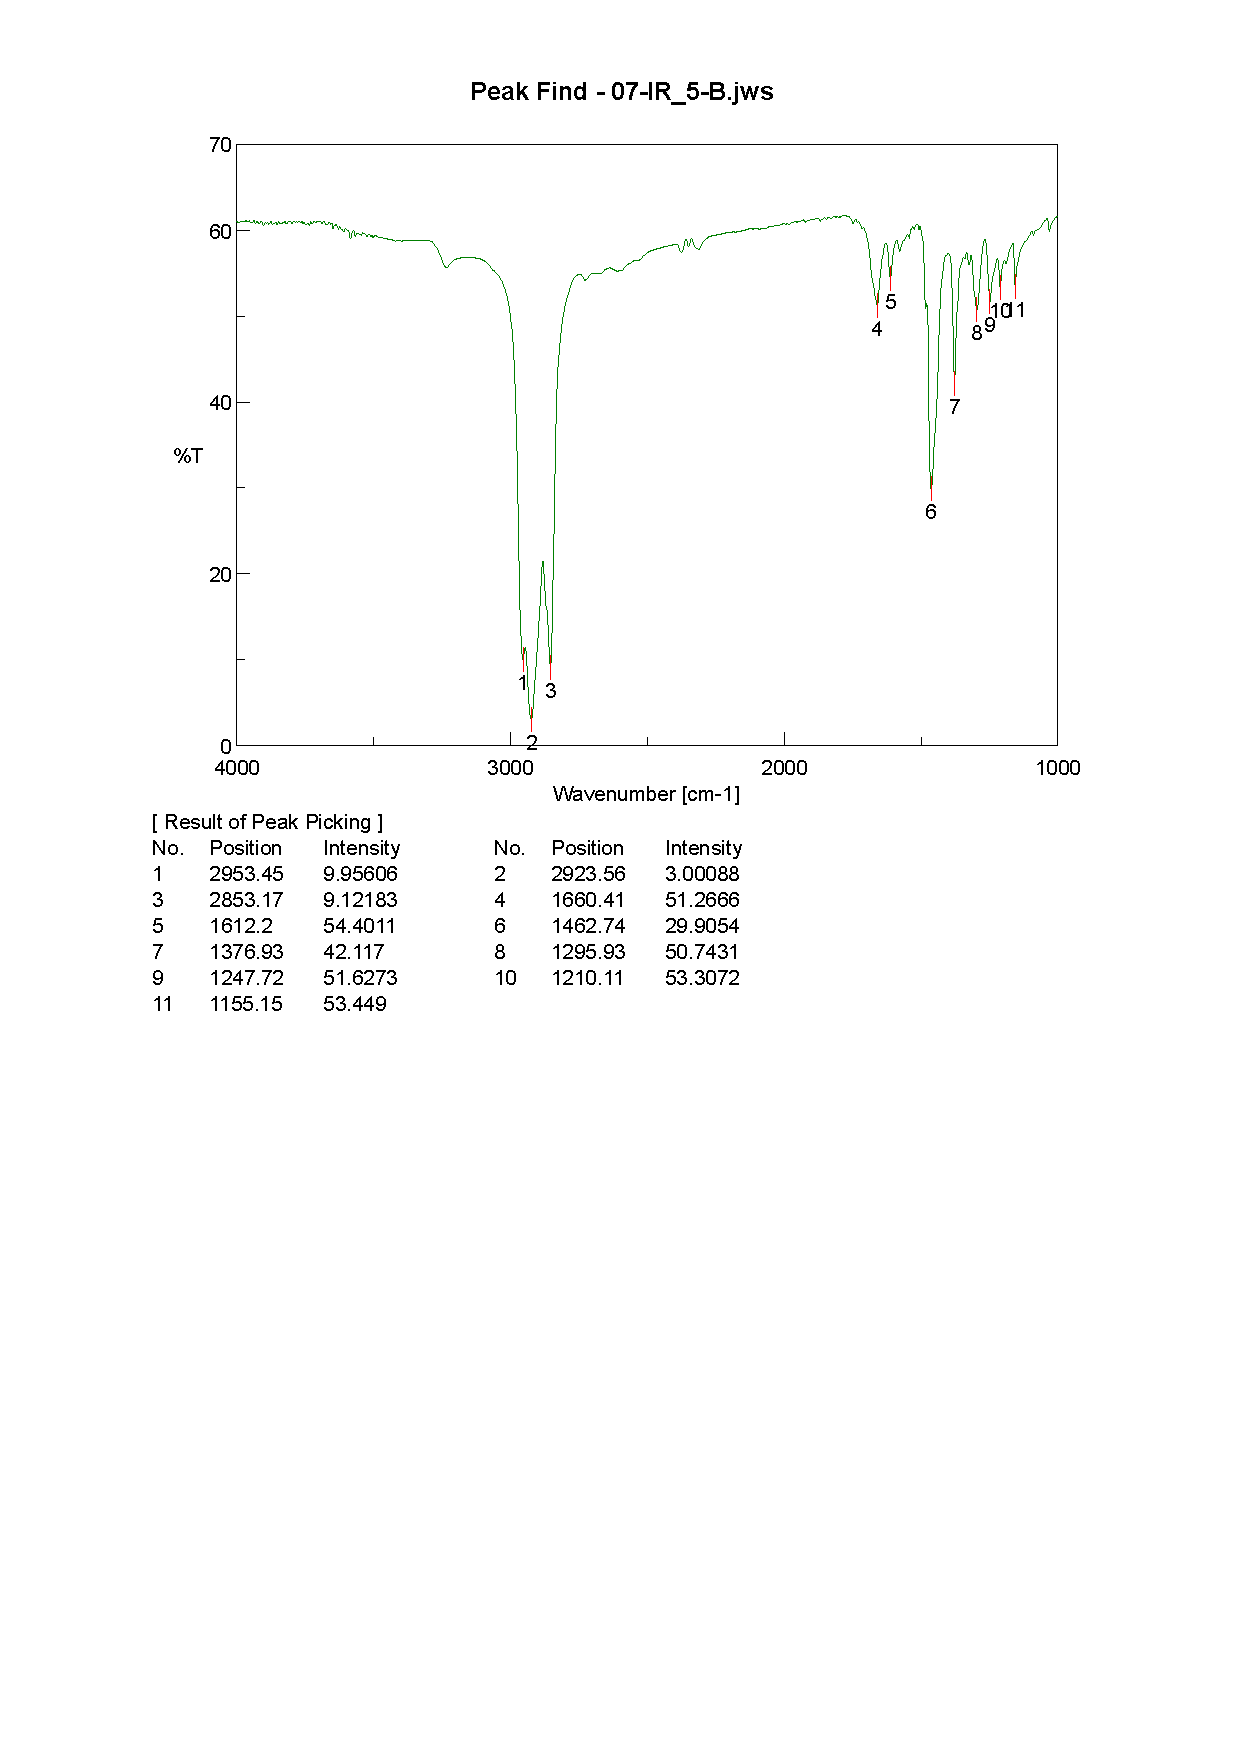
\includegraphics[width = 15 cm]{IR_5-1-B.pdf}
\caption{IR:5-1-B}
\label{IR_5-1-B}
\end{center}
\end{figure}

\begin{figure}[htbp]
\begin{center}
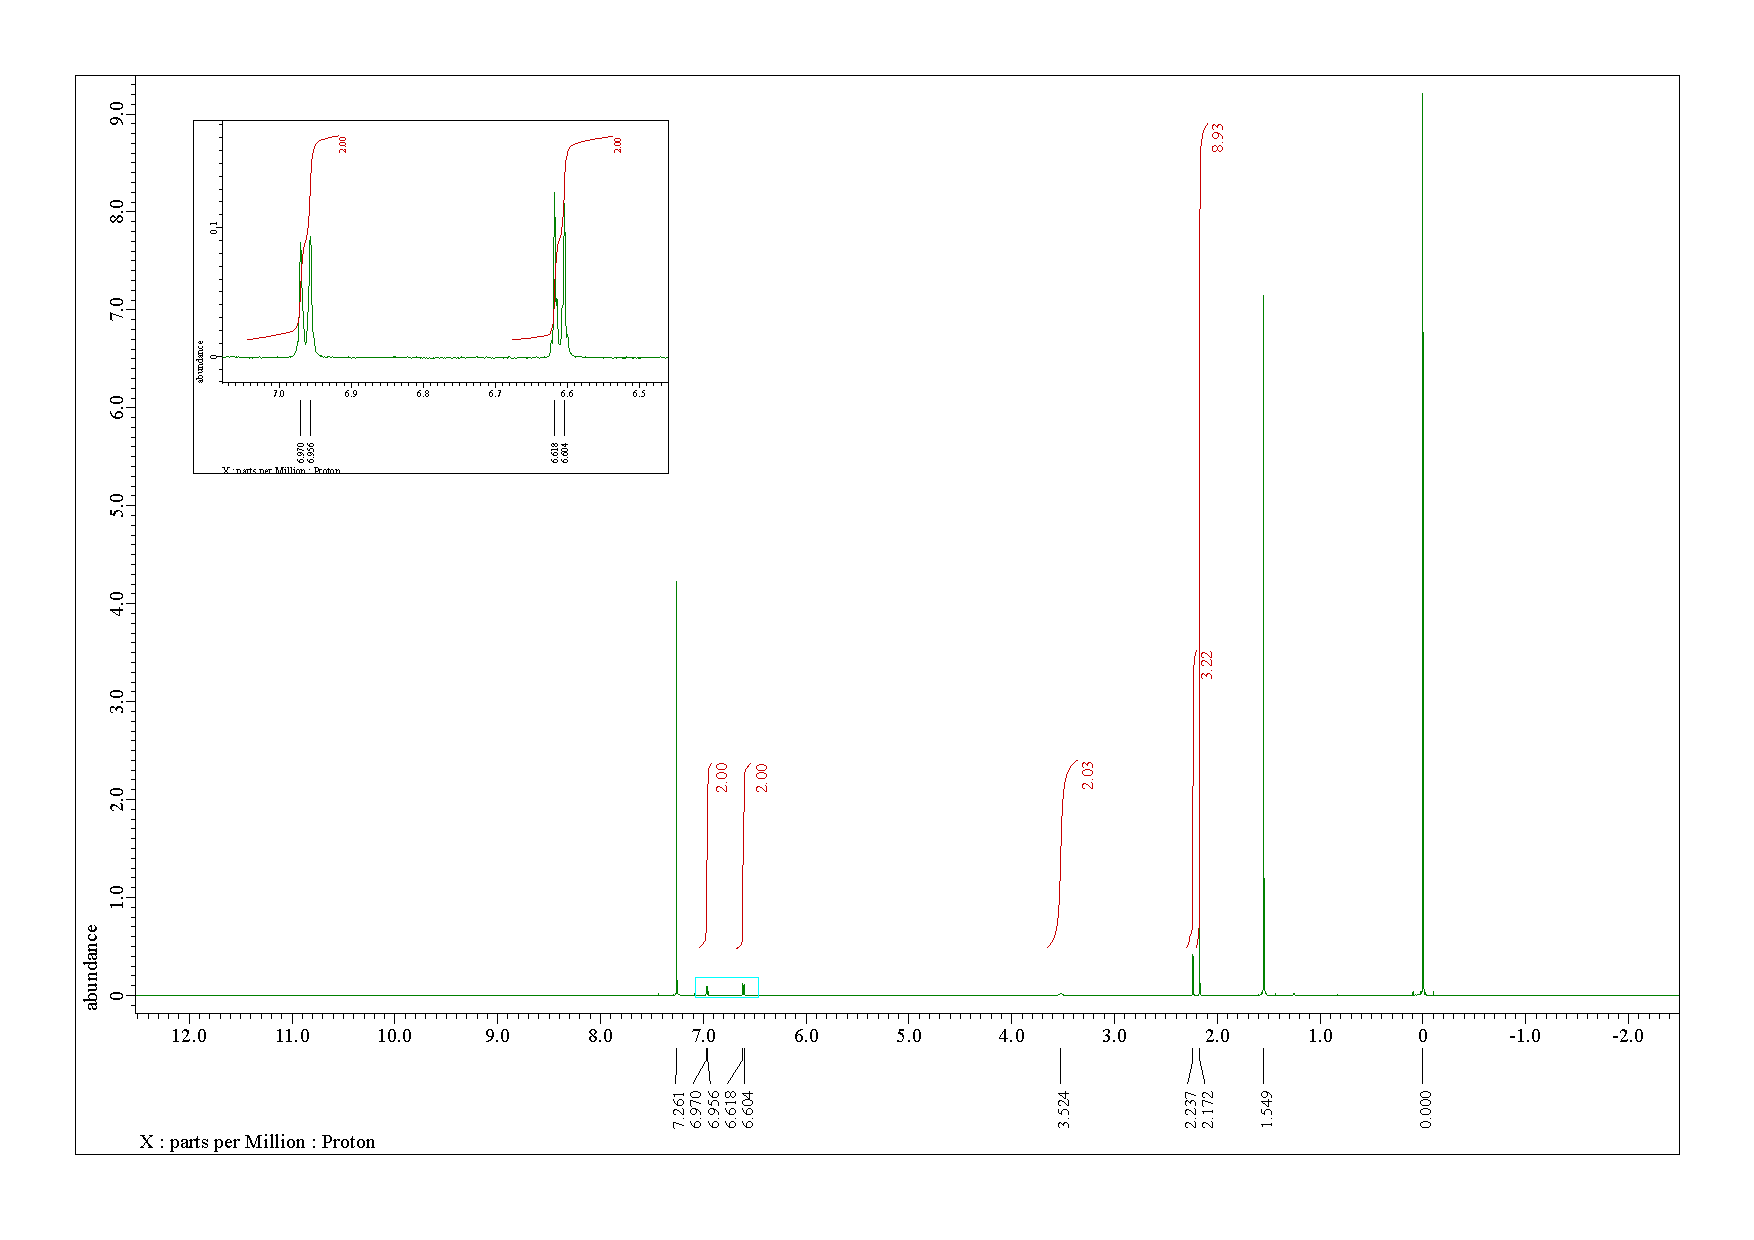
\includegraphics[width = 15 cm]{NMR_5-1-A-2.pdf}
\caption{\textbf{A}の誘導体の\ce{^1H} NMRスペクトル (\ce{CDCl3})}
\label{NMR_5-1-A-2}
\end{center}
\end{figure}




\end{document}